\documentclass[11pt]{article}
\usepackage[utf8]{inputenc}
\usepackage[T1]{fontenc}
\usepackage[margin=1in]{geometry}
\usepackage{lmodern}
\usepackage{microtype}
\usepackage{amsmath,amssymb}
\usepackage{booktabs}
\usepackage{natbib}
\usepackage[hidelinks]{hyperref}
\usepackage{url}
\usepackage{array}
\usepackage{xcolor}
\usepackage{tikz}
\usetikzlibrary{arrows.meta,positioning,shapes.geometric,fit,backgrounds,calc}
\usepackage{pgfplots}
\usepackage{pgfplotstable}
\pgfplotsset{compat=1.18}
\setlength{\emergencystretch}{3em}

% Every measured number below is a macro written by paper/make_numbers.py from results/.
% A value not measured yet prints as a bold "pending". Never type a number here.
% Plot data (figdata/*.csv) and the figure flags are written by paper/make_figures.py from results/.
% Rebuild with: uv run python paper/make_numbers.py && uv run python paper/make_figures.py
%               && (cd paper && tectonic fym1.tex)
% Voice: single author, first person singular ("I", "my"). tests/test_paper_voice.py guards it.
% Figures are TikZ/pgfplots source only: the public snapshot ships text files, no images.
% Generated by paper/make_numbers.py from results/. Do not edit by hand.
\newcommand{\fyDataThreads}{1}
\newcommand{\fyDataConversations}{192}
\newcommand{\fyDataIdentity}{\textbf{pending}}
\newcommand{\fyDataFormal}{\textbf{pending}}
\newcommand{\fyDataSynthetic}{\textbf{pending}}
\newcommand{\fyDataTrainExamples}{\textbf{pending}}
\newcommand{\fyDataKeptMessages}{436}
\newcommand{\fyGateBefore}{260}
\newcommand{\fyGateKept}{192}
\newcommand{\fyGateDropped}{68}
\newcommand{\fyGateDroppedNumber}{0}
\newcommand{\fyGateDroppedContact}{4}
\newcommand{\fyGateDroppedUnknown}{15}
\newcommand{\fyGateDroppedFakes}{56}
\newcommand{\fyGateReplaced}{353}
\newcommand{\fyGateFakesMedian}{2}
\newcommand{\fyGateFakesMax}{5}
\newcommand{\fySynthRaw}{2,500}
\newcommand{\fySynthKept}{1,319}
\newcommand{\fySynthGenerator}{McGill-NLP/AfriqueQwen3.5-9B-50Langs-Instruct-v1}
\newcommand{\fySynthLicence}{cc-by-4.0}
\newcommand{\fySynthDropUnknown}{932}
\newcommand{\fySynthDropLength}{211}
\newcommand{\fySynthDropNotMalagasy}{23}
\newcommand{\fySynthDropLeak}{3}
\newcommand{\fySynthChecked}{1,319}
\newcommand{\fySynthGateDropped}{35}
\newcommand{\fySynthGateKept}{1,284}
\newcommand{\fySynthGateStatus}{pass}
\newcommand{\fyBudgetR}{16}
\newcommand{\fyBudgetAlpha}{16}
\newcommand{\fyBudgetD}{12,288}
\newcommand{\fyBudgetK}{4,096}
\newcommand{\fyBudgetFull}{50,331,648}
\newcommand{\fyBudgetLora}{262,144}
\newcommand{\fyBudgetShare}{0.52\%}
\newcommand{\fySmokeVram}{9.8 GB}
\newcommand{\fyBaseModel}{McGill-NLP/AfriqueQwen3.5-9B-50Langs-Instruct-v1}
\newcommand{\fyModelSize}{9B}
\newcommand{\fyModelRepo}{Fan1000-Prog/fy-m1-9B}
\newcommand{\fyBaseLicense}{CC-BY-4.0}
\newcommand{\fyBaseLicenseHf}{cc-by-4.0}
\newcommand{\fyTrainGpu}{\textbf{pending}}
\newcommand{\fyTrainSteps}{\textbf{pending}}
\newcommand{\fyTrainEpochs}{\textbf{pending}}
\newcommand{\fyTrainTime}{\textbf{pending}}
\newcommand{\fyTrainLoss}{\textbf{pending}}
\newcommand{\fyEvalLoss}{\textbf{pending}}
\newcommand{\fyLoraR}{\textbf{pending}}
\newcommand{\fyLoraAlpha}{\textbf{pending}}
\newcommand{\fyLearningRate}{\textbf{pending}}
\newcommand{\fyLrScheduler}{\textbf{pending}}
\newcommand{\fyWarmupSteps}{\textbf{pending}}
\newcommand{\fyMaxSeqLen}{\textbf{pending}}
\newcommand{\fyEffectiveBatch}{\textbf{pending}}
\newcommand{\fyEvalPrompts}{\textbf{pending}}
\newcommand{\fyDriftBase}{\textbf{pending}}
\newcommand{\fyDriftFymOne}{\textbf{pending}}
\newcommand{\fyLeakFymOne}{\textbf{pending}}
\newcommand{\fyLeakMatches}{\textbf{pending}}
\newcommand{\fyLeakGeneric}{\textbf{pending}}
\newcommand{\fyLeakRejected}{\textbf{pending}}
\newcommand{\fyIdentityN}{\textbf{pending}}
\newcommand{\fyIdentityPassed}{\textbf{pending}}
\newcommand{\fyIdentityPassRate}{\textbf{pending}}
\newcommand{\fyIdentityThreshold}{\textbf{pending}}
\newcommand{\fyIdentityForeign}{\textbf{pending}}
\newcommand{\fyIdentityGate}{\textbf{pending}}
\newcommand{\fyPplBase}{\textbf{pending}}
\newcommand{\fyPplFymOne}{\textbf{pending}}
\newcommand{\fyBelebeleBase}{\textbf{pending}}
\newcommand{\fyBelebeleFymOne}{\textbf{pending}}
\newcommand{\fyChrfMgEnBase}{\textbf{pending}}
\newcommand{\fyChrfMgEnFymOne}{\textbf{pending}}
\newcommand{\fyChrfEnMgBase}{\textbf{pending}}
\newcommand{\fyChrfEnMgFymOne}{\textbf{pending}}
\newcommand{\fyJudgeModel}{\textbf{pending}}
\newcommand{\fyNaturalBase}{\textbf{pending}}
\newcommand{\fyNaturalFymOne}{\textbf{pending}}
\newcommand{\fyCorrectBase}{\textbf{pending}}
\newcommand{\fyCorrectFymOne}{\textbf{pending}}
\newcommand{\fyArenaVotes}{\textbf{pending}}
\newcommand{\fyArenaRaters}{\textbf{pending}}
\newcommand{\fyArenaWinRate}{\textbf{pending}}
\newcommand{\fyArenaCiLow}{\textbf{pending}}
\newcommand{\fyArenaCiHigh}{\textbf{pending}}
\newcommand{\fyTrimGates}{\textbf{pending}}
\newcommand{\fyVocabBefore}{\textbf{pending}}
\newcommand{\fyVocabAfter}{\textbf{pending}}
\newcommand{\fyParamsBefore}{\textbf{pending}}
\newcommand{\fyParamsAfter}{\textbf{pending}}
\newcommand{\fyGgufBefore}{\textbf{pending}}
\newcommand{\fyGgufAfter}{\textbf{pending}}
\newcommand{\fyTpsBefore}{\textbf{pending}}
\newcommand{\fyTpsAfter}{\textbf{pending}}
\newcommand{\fyCostVocabBefore}{248,077}
\newcommand{\fyCostVocabAfter}{74,040}
\newcommand{\fyCostTpwChatsBefore}{2.048}
\newcommand{\fyCostTpwChatsAfter}{2.077}
\newcommand{\fyCostTpwPromptsBefore}{2.269}
\newcommand{\fyCostTpwPromptsAfter}{2.302}
\newcommand{\fySelQwenBelebele}{66.7\%}
\newcommand{\fySelQwenBelebeleChat}{74.2\%}
\newcommand{\fySelQwenChrfMgEn}{56.2}
\newcommand{\fySelQwenChrfEnMg}{49.7}
\newcommand{\fySelQwenSecStep}{83.3}
\newcommand{\fySelQwenLicense}{CC-BY-4.0}
\newcommand{\fySelGemmaFourBelebele}{\textbf{pending}}
\newcommand{\fySelGemmaFourBelebeleChat}{75.0\%}
\newcommand{\fySelGemmaFourChrfMgEn}{\textbf{pending}}
\newcommand{\fySelGemmaFourChrfEnMg}{\textbf{pending}}
\newcommand{\fySelGemmaFourSecStep}{\textbf{pending}}
\newcommand{\fySelGemmaFourLicense}{Apache-2.0}
\newcommand{\fySelGemmaThreeBelebele}{69.7\%}
\newcommand{\fySelGemmaThreeBelebeleChat}{75.1\%}
\newcommand{\fySelGemmaThreeChrfMgEn}{51.8}
\newcommand{\fySelGemmaThreeChrfEnMg}{36.8}
\newcommand{\fySelGemmaThreeSecStep}{122.4}
\newcommand{\fySelGemmaThreeLicense}{Gemma Terms of Use}
\newcommand{\fyGreetQwenMean}{2.90}
\newcommand{\fyGreetQwenMalagasy}{95.0\%}
\newcommand{\fyGreetGemmaFourMean}{2.85}
\newcommand{\fyGreetGemmaFourMalagasy}{90.0\%}
\newcommand{\fyGreetGemmaThreeMean}{1.90}
\newcommand{\fyGreetGemmaThreeMalagasy}{80.0\%}
\newcommand{\fyGreetAnswers}{20}
\newcommand{\fyGreetJudge}{Claude Opus 5.5 (claude-opus-5-5), blind, run in Claude Code}
\newcommand{\fySelectionRows}{McGill-NLP/AfriqueQwen-8B & CC-BY-4.0 & \textbf{pending} & \textbf{pending} & \textbf{pending} & \textbf{pending} & 2.95 & \textbf{pending} \\ McGill-NLP/AfriqueQwen3.5-9B-50Langs-Instruct-v1 & CC-BY-4.0 & 66.7\% & 74.2\% & 56.2 & 49.7 & 2.83 & 2.90 \\ google/gemma-3-12b-it & Gemma Terms of Use & 69.7\% & 75.1\% & 51.8 & 36.8 & 2.79 & 1.90 \\ google/gemma-4-12B-it & Apache-2.0 & \textbf{pending} & 75.0\% & \textbf{pending} & \textbf{pending} & 2.79 & 2.85 \\}

% Generated by paper/make_figures.py from results/. Do not edit by hand.
\newcommand{\fyFigFunnelReady}{1}
\newcommand{\fyFigTrainReady}{0}


\definecolor{private}{RGB}{214,234,248}
\definecolor{gatecol}{RGB}{252,228,214}
\definecolor{traincol}{RGB}{226,239,218}
\tikzset{
  box/.style={draw, rounded corners=2pt, align=center, font=\footnotesize, inner sep=3pt,
              minimum height=2.2em, text width=#1},
  box/.default=2.3cm,
  flow/.style={-{Stealth[length=4pt]}, thick},
  ask/.style={draw, diamond, aspect=2.2, align=center, font=\scriptsize, inner sep=0.5pt, fill=gatecol},
  pendingbox/.style={draw, dashed, align=center, font=\footnotesize, text width=#1, minimum height=3.2cm},
}
\newcommand{\pendingplot}[2]{\tikz\node[pendingbox=#1]{\textbf{pending}\\[0.3em]#2};}

\title{fy-m1: Teaching an Open Model to Chat in Everyday Malagasy\\[0.3em]
  \large Version 0.1 --- full human ratings in v0.2}
\author{by Fandresena Raharinaivo}
\date{October 2026}

\begin{document}
\maketitle

\begin{abstract}
Open language models that cover Malagasy tend to answer like an official letter: formal, stiff, and often
half-translated from French or English. People in Madagascar do not text like that. I adapt an open
instruction model, \fyBaseModel{} \citep{afriqueqwen}, to everyday Malagasy chat with QLoRA on a single
GPU. The training mix combines \fyGateKept{} real family conversations that passed a strict automatic
anonymisation gate, \fySynthGateKept{} synthetic chats that the base model itself wrote from few-shot
real examples, short formal chats built from Malagasy Wikipedia, and identity chats that I wrote myself.
I describe the privacy pipeline in full, because it is designed so that no person reads the private text,
and I release the code, the evaluation prompts and every measured value through a script. The evaluation
measures drift into full French or English, blind LLM-judge scores, a leak gate, an identity gate, and
regressions on reading (Belebele) and translation (FLORES+). This is version 0.1: the base-model
comparison, the data counts and the tokenizer trimming cost are measured; the fine-tuned model's scores
print as ``pending'' until their result files exist, and the blind human comparison reports only early
votes. No private text is released.
\end{abstract}

\section{Introduction}
\label{sec:intro}
Malagasy is the national language of Madagascar, but most
Malagasy text online is formal: news, Wikipedia, religious and government writing. Models trained on
that text learn that register. When a user writes a short, casual message, they get back a polished
paragraph that no one would send to a friend.

Everyday Malagasy looks different. French words are mixed in freely, including French verbs used with
Malagasy grammar (``lancer-na''). Spelling is phonetic and shortened (``zany'' for ``izany''). Replies
are short, with humour and emoji. This is code-switching in the sense of \citet{dogruoz-etal-2021-survey},
and for this project it is the target, not an error: a reply counts as drifting only if it is entirely
French or English with no Malagasy in it.

My goal is modest and measurable: a model that is clearly better than its base model at everyday
Malagasy chat, without losing much general Malagasy ability, trained on one GPU, served for free on a
CPU, and released under a simple open licence. The constraint that shapes everything else is privacy:
the only source of the target style is private family chat, and the people in it agreed to its use on
the condition that nobody reads it. The contributions are:
\begin{enumerate}
  \item a base-model comparison for Malagasy chat on a free 16\,GB T4 GPU, with one Belebele protocol
        for every candidate and a licence rule stated up front (Section~\ref{sec:selection});
  \item a privacy-first data pipeline in which no person reads the cleaned chats: anonymisation, a
        strict automatic gate that fails closed, a strict automatic gate on the synthetic chats, and a
        leak gate on the trained model (Sections~\ref{sec:data} and~\ref{sec:gates});
  \item fy-m1 itself, with every number in this paper written by a script from a measured output file,
        so that a value not measured yet cannot appear.
\end{enumerate}
Figure~\ref{fig:pipeline} shows the whole pipeline.

\begin{figure}[t]
\centering
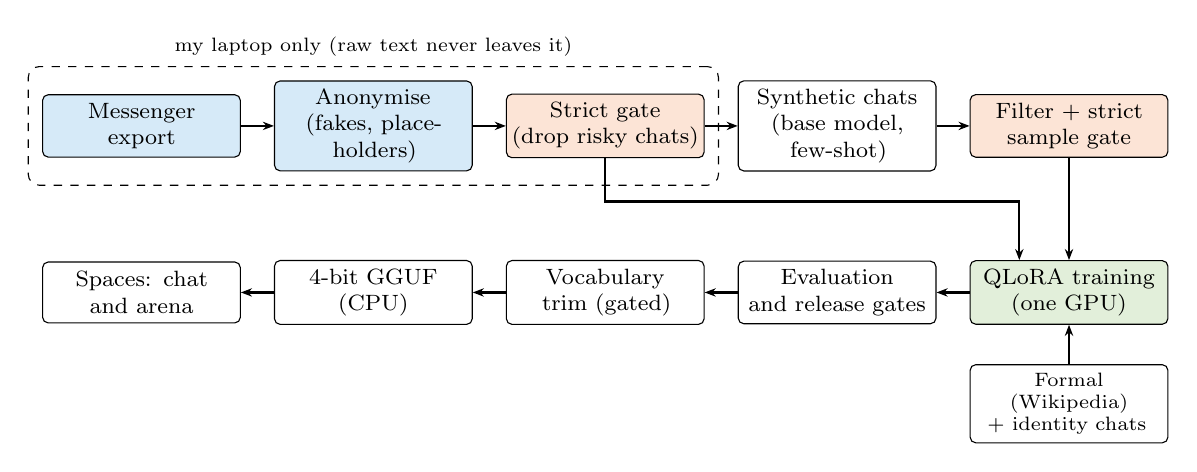
\begin{tikzpicture}[node distance=0.5cm and 0.42cm]
  \node[box, fill=private] (export) {Messenger\\export};
  \node[box, fill=private, right=of export] (anon) {Anonymise\\(fakes, placeholders)};
  \node[box, fill=gatecol, right=of anon] (gate) {Strict gate\\(drop risky chats)};
  \node[box, right=of gate] (synth) {Synthetic chats\\(base model, few-shot)};
  \node[box, fill=gatecol, right=of synth] (sgate) {Filter + strict\\sample gate};
  \node[box, fill=traincol, below=1.3cm of sgate] (train) {QLoRA training\\(one GPU)};
  \node[box, left=of train] (eval) {Evaluation\\and release gates};
  \node[box, left=of eval] (trim) {Vocabulary\\trim (gated)};
  \node[box, left=of trim] (gguf) {4-bit GGUF\\(CPU)};
  \node[box, left=of gguf] (spaces) {Spaces: chat\\and arena};
  \node[box, below=0.5cm of train, font=\scriptsize] (extra) {Formal (Wikipedia)\\+ identity chats};
  \begin{scope}[on background layer]
    \node[draw, dashed, rounded corners, fit=(export)(anon)(gate), inner sep=5pt,
          label={[font=\scriptsize]above:my laptop only (raw text never leaves it)}] (laptop) {};
  \end{scope}
  \draw[flow] (export) -- (anon);
  \draw[flow] (anon) -- (gate);
  \draw[flow] (gate) -- (synth);
  \draw[flow] (synth) -- (sgate);
  \draw[flow] (sgate) -- (train);
  \draw[flow] (gate.south) -- ++(0,-0.55) -| ($(train.north west)!0.25!(train.north east)$);
  \draw[flow] (extra) -- (train);
  \draw[flow] (train) -- (eval);
  \draw[flow] (eval) -- (trim);
  \draw[flow] (trim) -- (gguf);
  \draw[flow] (gguf) -- (spaces);
\end{tikzpicture}
\caption{The fy-m1 pipeline. Blue steps run only on my laptop; orange steps are strict automatic gates
that drop data instead of asking a person to read it. The real chats that pass the gate feed training
directly and also serve as few-shot examples for the synthetic chats. The leak gate (Section~\ref{sec:gates}) compares the trained
model's answers with the real chats before release.}
\label{fig:pipeline}
\end{figure}

\section{Related work}
\label{sec:related}
\paragraph{Malagasy in multilingual models.} Malagasy is covered by large multilingual benchmarks such as
Belebele \citep{bandarkar-etal-2024-belebele} and FLORES \citep{goyal-etal-2022-flores,nllb2022}, now
maintained as FLORES+ \citep{burchell-etal-2024-findings,floresplus}. Recent open models list Malagasy
among their languages, including the Gemma family \citep{gemma3,gemma4} and AfriqueQwen, a Qwen-based
model adapted to African languages \citep{afriqueqwen}; multilingual instruction tuning at scale is
studied by \citet{ustun-etal-2024-aya}. These benchmarks measure formal reading and translation; none
measures casual chat, and I know of no public evaluation of informal, code-switched Malagasy.

\paragraph{Code-switching.} Mixing languages within a conversation is the normal way many multilingual
communities write, yet language technologies often treat it as noise \citep{dogruoz-etal-2021-survey}.
I take the opposite view for Malagasy--French and define drift only as a full switch away from Malagasy.

\paragraph{Parameter-efficient fine-tuning.} LoRA \citep{hu2022lora} learns a low-rank update next to a
frozen weight matrix; QLoRA \citep{dettmers2023qlora} stores the frozen model in 4-bit NormalFloat (NF4),
so a model of about ten billion parameters trains on one 16\,GB GPU. I use Unsloth \citep{unsloth}, an
implementation of the same method with lower memory use, and a cosine learning-rate decay
\citep{loshchilov2017sgdr} after a short linear warmup.

\paragraph{Synthetic data.} Prompting a model to write its own training data is an established way to
bootstrap instruction data \citep{wang-etal-2023-self}. Training a model repeatedly on its own outputs
can narrow its output distribution \citep{shumailov2024collapse}. My synthetic chats come from the base
model itself (one round, few-shot prompted with real chats), so this risk applies; I discuss it in
Section~\ref{sec:limitations}.

\paragraph{Privacy.} Text anonymisation is hard to do completely, and masking named entities alone does
not remove all identifying information \citep{lison-etal-2021-anonymisation}. Language models can also
emit verbatim training text \citep{carlini2021extracting}. I therefore combine anonymisation with gates
that drop, rather than repair, anything uncertain, and with a verbatim-overlap check on the trained model.

\paragraph{Evaluation and compression.} LLM judges are a cheap proxy for human preference
\citep{zheng2023judging}; I use one blind and treat it as a signal, not a verdict. Language ID uses
GlotLID \citep{kargaran-etal-2023-glotlid}, translation uses chrF++ \citep{popovic-2017-chrf}.
Vocabulary trimming follows \citet{ushio-etal-2023-efficient}; layer pruning
\citep{gromov2024deeper} is left for later.

\section{Data}
\label{sec:data}
I describe the data but do not share it: part of it is private conversations. Only counts are
published (\path{results/data_stats.json}, \path{results/data_gate.json},
\path{results/synth_stats.json}, \path{results/synth_gate.json}). Figure~\ref{fig:funnel} shows how
much data survives each step.

\begin{figure}[t]
\centering
\ifnum\fyFigFunnelReady=1
\begin{tikzpicture}
\begin{axis}[
  xbar, width=0.74\linewidth, height=5.2cm, bar width=9pt, xmin=0,
  y dir=reverse, enlarge y limits=0.14, enlarge x limits={upper, value=0.16},
  symbolic y coords={real-cleaned,real-kept,synth-raw,synth-filtered,synth-kept},
  ytick=data,
  yticklabels={Real: cleaned, Real: passed strict gate, Synthetic: written, Synthetic: kept by filter,
               Synthetic: passed sample gate},
  yticklabel style={font=\footnotesize}, xticklabel style={font=\footnotesize},
  xlabel={Conversations}, xlabel style={font=\footnotesize},
  scaled x ticks=false, /pgf/number format/1000 sep={{{{,}}}},
  point meta=x, nodes near coords={\pgfmathprintnumber[1000 sep={{{{,}}}}]{\pgfplotspointmeta}},
  nodes near coords style={font=\footnotesize, anchor=west}, axis lines*=left]
\addplot[draw=black, fill=traincol] table[col sep=comma, x=count, y=id]{figdata/funnel.csv};
\end{axis}
\end{tikzpicture}
\else
\pendingplot{8cm}{the data funnel needs results/data\_gate.json, synth\_stats.json and synth\_gate.json}
\fi
\caption{Data funnel (\texttt{paper/figdata/funnel.csv}, written by \texttt{paper/make\_figures.py} from
\texttt{results/}). Real: \fyGateBefore{} cleaned conversations, \fyGateKept{} passed the strict gate.
Synthetic: \fySynthRaw{} written, \fySynthKept{} kept by the automatic filter, \fySynthGateKept{} passed
the strict sample gate. Every step drops data on purpose; the formal and identity slices are not shown.}
\label{fig:funnel}
\end{figure}

\paragraph{Real chats.} The main source is one family's Messenger export (threads used: \fyDataThreads{}).
Every sender's side is used as the assistant in turn. A local script splits the export into short
multi-turn conversations at long gaps, merges back-to-back messages from the same sender, and replaces
names, nicknames (also inside message text and handles), phone numbers, emails, links and addresses with
fakes or placeholders (\path{docs/anonymisation.md}).

\paragraph{Strict automatic gate.} No person reads the cleaned text; a strict automatic gate replaces the
manual review I first planned. Figure~\ref{fig:gate} shows its decisions. At the word level, a word is
kept only if a known-word list has it: common Malagasy words, Malagasy Wikipedia vocabulary
\citep{wikipedia-dump}, Malagasy web text from HPLT~2.0 \citep{hplt2}, a short hand list of places and
brands, and French and English words from \texttt{wordfreq} \citep{wordfreq}. French first names from
INSEE \citep{insee-prenoms} never count as known words. In a name position (mid-sentence or after a
person marker such as \emph{i} or \emph{ry}) only the hand list can clear a word. Any other word is
replaced with a fake name. At the conversation level the gate drops the whole conversation for a long
digit run (a possible phone number), an email, link or handle, a hidden character, more than 30\% of
words replaced, or more than five fake names. Of \fyGateBefore{} cleaned conversations it dropped
\fyGateDropped{} (a conversation can count under more than one reason): \fyGateDroppedNumber{} for a
long digit run, \fyGateDroppedContact{} for a contact, \fyGateDroppedUnknown{} for too many unknown words
and \fyGateDroppedFakes{} for too many fake names. The gate over-masks on purpose: \fyGateReplaced{} words
were replaced in total, a median of \fyGateFakesMedian{} and at most \fyGateFakesMax{} per kept
conversation. \fyGateKept{} conversations (\fyDataKeptMessages{} messages) passed.

\begin{figure}[t]
\centering
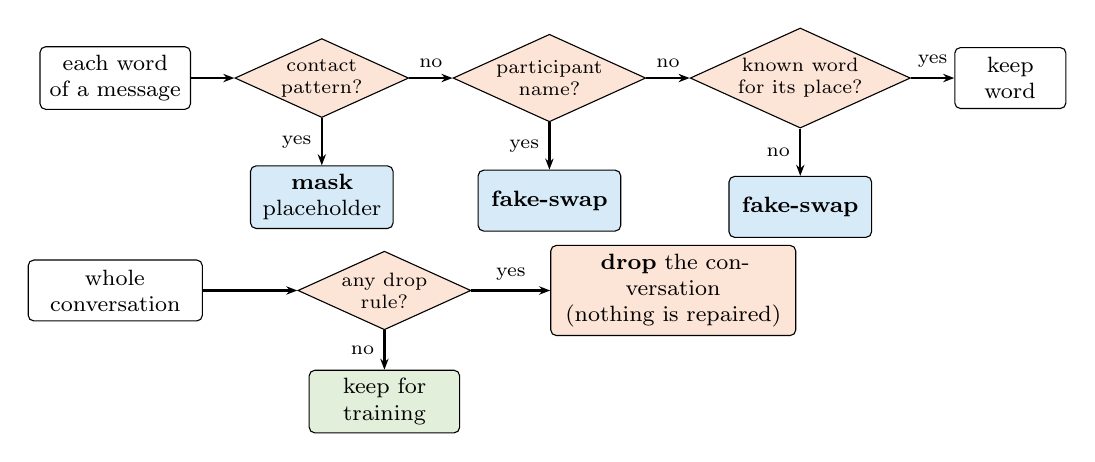
\begin{tikzpicture}[node distance=0.5cm and 0.55cm]
  \node[box=1.7cm] (tok) {each word\\of a message};
  \node[ask, right=of tok] (contact) {contact\\pattern?};
  \node[ask, right=of contact] (name) {participant\\name?};
  \node[ask, right=of name] (known) {known word\\for its place?};
  \node[box=1.6cm, below=0.6cm of contact, fill=private] (mask) {\textbf{mask}\\placeholder};
  \node[box=1.6cm, below=0.6cm of name, fill=private] (fake1) {\textbf{fake-swap}};
  \node[box=1.6cm, below=0.6cm of known, fill=private] (fake2) {\textbf{fake-swap}};
  \node[box=1.2cm, right=of known] (keepw) {keep\\word};
  \node[box=2.0cm, below=1.9cm of tok] (conv) {whole\\conversation};
  \node[ask, right=1.2cm of conv] (rules) {any drop\\rule?};
  \node[box=2.9cm, right=1.0cm of rules, fill=gatecol] (drop) {\textbf{drop} the conversation\\(nothing is repaired)};
  \node[box=1.7cm, below=0.5cm of rules, fill=traincol] (keepc) {keep for\\training};
  \draw[flow] (tok) -- (contact);
  \draw[flow] (contact) -- node[above, font=\scriptsize]{no} (name);
  \draw[flow] (name) -- node[above, font=\scriptsize]{no} (known);
  \draw[flow] (known) -- node[above, font=\scriptsize]{yes} (keepw);
  \draw[flow] (contact) -- node[left, font=\scriptsize]{yes} (mask);
  \draw[flow] (name) -- node[left, font=\scriptsize]{yes} (fake1);
  \draw[flow] (known) -- node[left, font=\scriptsize]{no} (fake2);
  \draw[flow] (conv) -- (rules);
  \draw[flow] (rules) -- node[above, font=\scriptsize]{yes} (drop);
  \draw[flow] (rules) -- node[left, font=\scriptsize]{no} (keepc);
\end{tikzpicture}
\caption{The privacy decisions, with no real example. Top: per word, the anonymiser masks contact
patterns (phone, email, link, handle, address) with a placeholder and swaps participant names and
nicknames for fakes; the strict gate then swaps any word that no known-word list clears for its position.
Bottom: per conversation, the gate drops the whole conversation if any rule fires (long digit run,
contact left, hidden character, more than 30\% of words replaced, more than five fakes).}
\label{fig:gate}
\end{figure}

\paragraph{Synthetic chats.} Real chats are far too few on their own, so an open model that I run myself
writes everyday chats, few-shot prompted with cleaned real chats. Only permissively licensed generators are
allowed, because synthetic chats are training data and their licence reaches fy-m1: the code refuses any
other. The generator was \fySynthGenerator{} (licence \fySynthLicence{}), which is also the base model,
so this step distils the style of the few-shot real examples back into the same model. An automatic
filter kept \fySynthKept{} of \fySynthRaw{} generated chats; the largest drop reasons were a word that no
list clears in a name position (\fySynthDropUnknown{}), a length outside the allowed range
(\fySynthDropLength{}), no Malagasy in a reply (\fySynthDropNotMalagasy{}), and an 8-word overlap with the
real chats (\fySynthDropLeak{}). A strict automatic sample gate then checked all \fySynthChecked{} kept
chats for leftover real names, contacts, numbers, drift and broken turns, and dropped \fySynthGateDropped{}
(status: \fySynthGateStatus{}), leaving \fySynthGateKept{}. No closed-API model output is in the
training data.

\paragraph{Formal slice.} \fyDataFormal{} short ``tell me about'' chats built from Malagasy Wikipedia
paragraphs, so facts and standard spelling survive. The slice is kept small so it does not pull the
style back to formal.

\paragraph{Identity chats.} \fyDataIdentity{} short exchanges, which I wrote in my own words, answer
``who are you?'' consistently (fy-m1, made by Fan's lab, built on an open model) and politely refuse
harmful requests.

In total the model trained on \fyDataTrainExamples{} examples (\fyDataSynthetic{} synthetic).

\paragraph{Consent and privacy of the data.} Everyone in the conversations consented to their messages
being used. The raw export never left my laptop; no person read the cleaned text, and only conversations
that passed the strict gate were used. The cleaned data lives in a private dataset and is not released.
The anonymiser has known limits, listed in \path{docs/anonymisation.md} and pinned as expected-failure
tests: names of people outside the chat typed as plain text, a name that is also an everyday word at the
start of a sentence, phone numbers written in words or split over two messages, and some addresses and
place names. The strict gate and the leak gate (Section~\ref{sec:gates}) are the backstops for these.

\section{Method}
\label{sec:method}
\subsection{Choosing the base model}
\label{sec:selection}
I compared open instruction models that fit QLoRA training on a 16\,GB T4 GPU, the free GPU on Kaggle
and Colab. Each candidate was loaded in 4-bit and scored on: reading comprehension (Belebele,
\texttt{plt\_Latn}), both as plain-text 0-shot completion (one protocol for every candidate) and in the
model's chat format; translation in both directions with English (FLORES+ devtest, chrF++); tokens per
Malagasy word; a short QLoRA smoke run on a T4 (wall time per step); and a blind greeting gate, in which
the judge of Section~\ref{sec:metrics} scored \fyGreetAnswers{} everyday greeting answers per model with
model names hidden. A licence rule comes first: fy-m1 ships under a simple open licence, so the base must
have one. Section~\ref{sec:res-selection} gives the measured values and the choice.

\subsection{Fine-tuning with QLoRA}
\label{sec:training}
\paragraph{Adapters.} For a frozen weight matrix $W_0 \in \mathbb{R}^{d \times k}$ of the base model,
LoRA \citep{hu2022lora} learns $A \in \mathbb{R}^{r \times k}$ and $B \in \mathbb{R}^{d \times r}$ with
rank $r \ll \min(d, k)$ and computes
\begin{equation}
  h = W_0 x + \frac{\alpha}{r} B A x ,
  \label{eq:lora}
\end{equation}
where $\alpha$ is a fixed scale. $B$ starts at zero, so training starts from the base model exactly. QLoRA
\citep{dettmers2023qlora} stores $W_0$ in 4-bit NF4 and dequantises it on the fly; only $A$ and $B$ get
gradients and optimiser state. A full update of $W_0$ trains $dk$ weights, an adapter $r(d+k)$
(Figure~\ref{fig:qlora}). The adapter settings are rank $r=\fyBudgetR{}$ and $\alpha=\fyBudgetAlpha{}$
(\path{results/lora_budget.json}, read from the training notebook's settings), on the attention and MLP
projections of the language layers, using Unsloth \citep{unsloth}. The base model is a hybrid: most of
its layers use linear attention, interleaved with full-attention layers. Unsloth chooses which projections
of each layer type get adapters, and the training log does not record the total trainable count, so I
report the per-matrix size only.

\begin{figure}[t]
\centering
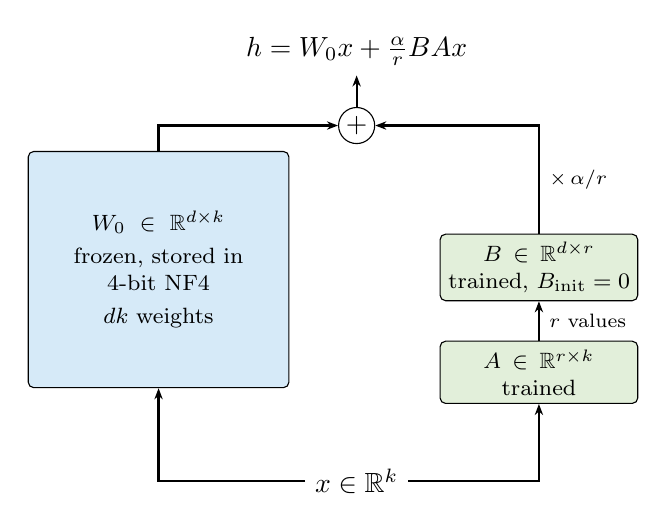
\begin{tikzpicture}[node distance=0.5cm]
  \node (x) {$x \in \mathbb{R}^{k}$};
  \node[box=3.1cm, fill=private, above left=0.9cm and 0.2cm of x, minimum height=3.0cm] (W)
       {$W_0 \in \mathbb{R}^{d\times k}$\\[0.3em]frozen, stored in\\4-bit NF4\\[0.3em]$dk$ weights};
  \node[box=2.3cm, fill=traincol, above right=0.7cm and 0.4cm of x] (A) {$A \in \mathbb{R}^{r\times k}$\\trained};
  \node[box=2.3cm, fill=traincol, above=0.5cm of A] (B) {$B \in \mathbb{R}^{d\times r}$\\trained, $B_{\text{init}}=0$};
  \node[draw, circle, inner sep=1pt, above=4.0cm of x] (plus) {$+$};
  \node[above=0.4cm of plus] (h) {$h = W_0x + \tfrac{\alpha}{r}BAx$};
  \draw[flow] (x) -| (W.south);
  \draw[flow] (x) -| (A.south);
  \draw[flow] (A) -- node[right, font=\scriptsize]{$r$ values} (B);
  \draw[flow] (B.north) |- node[pos=0.25, right, font=\scriptsize]{$\times\,\alpha/r$} (plus.east);
  \draw[flow] (W.north) |- (plus.west);
  \draw[flow] (plus) -- (h);
\end{tikzpicture}
\caption{QLoRA on one weight matrix. Only $A$ and $B$ are trained, $r(d+k)$ weights. Example from the base
model's configuration (\texttt{results/lora\_budget.json}): an MLP up-projection has
$d=\fyBudgetD{}$, $k=\fyBudgetK{}$, so $dk=\fyBudgetFull{}$ weights; a rank-\fyBudgetR{} adapter trains
\fyBudgetLora{} of them (\fyBudgetShare{}). Peak GPU memory in the T4 smoke run was \fySmokeVram{}
(\texttt{results/model\_selection.json}); the training run's peak memory was not logged.}
\label{fig:qlora}
\end{figure}

\paragraph{Objective.} Each training example is one conversation rendered in the base model's own chat
template, with thinking turned off and a fixed Malagasy system prompt that names the model. Let
$y=(y_1,\dots,y_{T_y})$ be its tokens and $m^{y}_t \in \{0,1\}$ a mask that is $1$ exactly on the tokens of assistant
replies (each reply's end-of-turn token included; system prompt, user turns and assistant headers
excluded). For a batch $\mathcal{B}$ of conversations (all micro-batches of one optimiser step under
gradient accumulation), training minimises the next-token cross-entropy summed over every assistant token
in the batch and divided by the number of those tokens,
\begin{equation}
  \mathcal{L}(A, B) = -\frac{1}{\sum_{y \in \mathcal{B}} \sum_{t} m^{y}_t}
  \sum_{y \in \mathcal{B}} \sum_{t=1}^{T_y} m^{y}_t \log p_{W_0, A, B}\left(y_t \mid y_{<t}\right),
  \label{eq:loss}
\end{equation}
so each assistant token weighs the same, whatever conversation it sits in (Figure~\ref{fig:mask}). The template's generation prompt puts an
empty thinking block after the assistant header; every assistant turn in training carries the same block,
so the model learns the turn format it sees when it answers.

\begin{figure}[t]
\centering
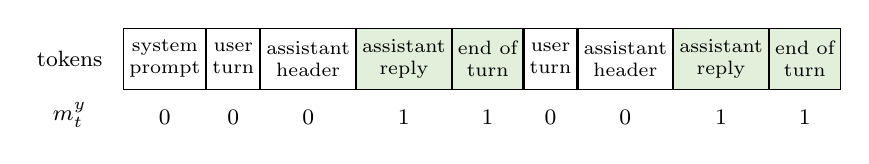
\begin{tikzpicture}[tok/.style={draw, font=\scriptsize, minimum height=2.2em, inner sep=2pt, align=center}]
  \node[font=\footnotesize] (lab) {tokens};
  \node[tok, right=4pt of lab] (s) {system\\prompt};
  \node[tok, right=0pt of s] (u1) {user\\turn};
  \node[tok, right=0pt of u1] (h1) {assistant\\header};
  \node[tok, fill=traincol, right=0pt of h1] (a1) {assistant\\reply};
  \node[tok, fill=traincol, right=0pt of a1] (e1) {end of\\turn};
  \node[tok, right=0pt of e1] (u2) {user\\turn};
  \node[tok, right=0pt of u2] (h2) {assistant\\header};
  \node[tok, fill=traincol, right=0pt of h2] (a2) {assistant\\reply};
  \node[tok, fill=traincol, right=0pt of a2] (e2) {end of\\turn};
  \node[font=\footnotesize, below=6pt of lab] {$m^{y}_t$};
  \foreach \n/\m in {s/0,u1/0,h1/0,a1/1,e1/1,u2/0,h2/0,a2/1,e2/1}
    \node[font=\footnotesize, below=4pt of \n] {$\m$};
\end{tikzpicture}
\caption{Assistant-only loss over the chat template (schematic, no real text). Green tokens have
$m^{y}_t=1$ and count in Equation~\ref{eq:loss}; the rest are context only. Each assistant header includes
the template's empty thinking block.}
\label{fig:mask}
\end{figure}

\paragraph{Optimisation.} Training uses an 8-bit AdamW optimiser, a learning rate of \fyLearningRate{}
with a \fyLrScheduler{} schedule and \fyWarmupSteps{} linear warmup steps, sequence length
\fyMaxSeqLen{}, effective batch size \fyEffectiveBatch{}, and a plan of \fyTrainEpochs{} epochs
(\fyTrainPlannedSteps{} steps); these values are read back from the run's own log
(\path{results/train_log.json}). A small held-out share of the
conversations gives an evaluation loss at every checkpoint; training stops early when that loss rises at
two evaluations in a row, and the checkpoint with the best evaluation loss is kept. Notebook sessions can
disconnect, so checkpoints go to a private repository and a new session resumes from the latest one; a
run refuses to resume if its settings or code changed. Training code reaches the GPU only as a synced
copy of the clean main branch.

\subsection{Making the model smaller: vocabulary trimming}
\label{sec:trim}
Much of a multilingual model's vocabulary is for scripts and languages fy-m1 never uses. Following
\citet{ushio-etal-2023-efficient}, I keep only the tokens seen in public Malagasy, French and English
text (Wikipedia and HPLT~2.0, never the private chats) plus all special and byte-fallback tokens, and drop
the matching embedding and output rows. The trim ships only if it passes three gates: held-out Malagasy
text round-trips through the new tokenizer unchanged; greedy answers are unchanged for at least 95\% of the
test prompts; and Belebele stays within one point. Removing whole layers \citep{gromov2024deeper} would
save more but needs healing with extra training; I leave it for v0.2.

\section{Experiments}
\label{sec:experiments}
\subsection{Compute}
\label{sec:compute}
Two kinds of GPU were used. Free T4 GPUs on Kaggle and Google Colab ran the base-model baselines, the
synthetic-chat generation and the QLoRA smoke tests of Section~\ref{sec:selection}. Training and
evaluation of fy-m1 run on a paid Colab Pro A100 GPU; the training log records the GPU that was actually
used (\fyTrainGpu{}, \path{results/train_log.json}). The demo runs on a free CPU.

\subsection{Test set and metrics}
\label{sec:metrics}
I generated answers from the base model and fy-m1 to \fyEvalPrompts{} fresh everyday prompts with the
same system prompt and sampling settings. The prompts were written fresh, not taken from the chats, so
the test set holds no private text and is public (\path{eval/prompts.jsonl}).

\paragraph{Drift.} A reply counts as Malagasy if GlotLID \citep{kargaran-etal-2023-glotlid} says so, or
if at least a tenth of its words are common Malagasy words; mixed Malagasy--French passes. A reply that
is fully French or English drifts. The drift rate is the share of replies that drift.

\paragraph{LLM judge.} An LLM judge scored both answer sets blind, with labels hidden and order shuffled,
on a published 1--5 rubric for naturalness and correctness \citep{zheng2023judging}. Methods disclosure:
the judge is \fyJudgeModel{}; rubric in \path{src/fym1/eval/judge_rubric.md}. The greeting gate of
Section~\ref{sec:selection} used the same rubric with \fyGreetJudge{}. The judge sees only the public
prompts and the models' answers, never the private chats, and its outputs are never training data. Judge
scores are a cheap signal, not a substitute for native speakers.

\paragraph{Regression checks.} Belebele accuracy, FLORES+ chrF++ in both directions, and held-out chat
perplexity should not get much worse after fine-tuning.

\subsection{Release gates}
\label{sec:gates}
\paragraph{Leak gate.} Any fy-m1 answer that shares a run of 8 words with the real training chats blocks
release, as a simple test for verbatim memorisation \citep{carlini2021extracting}. The check is strict and
automatic: only the matched words are looked at, never the chat around them, and any rejected run means
fixing the data, filtering or retraining.

\paragraph{Identity check.} A second strict, automatic gate covers the identity and safety prompts of the
test set plus extra identity prompts in Malagasy, some mixed with French (\path{eval/identity_check.jsonl}).
A reply passes when it is Malagasy (the drift test above) and names itself fy-m1 or Fan's lab as the
prompt asks. Mentions of other models and companies are judged in two tiers. A \emph{hard fail}, on any
prompt, is an explicit false self-claim: another model's or company's name in a self-identification shape
(``I am \ldots'', ``my name is \ldots'', ``made by \ldots'' with the model as subject, in Malagasy, French
or English), unless the shape is negated or only repeats the user's question. One hard fail fails the
gate. An \emph{ordinary miss}, only on prompts about the model itself, is any other unexcused mention of
such a name; a denial or a repeated question excuses it. The split keeps the hard fail for clear lies
about identity, while fuzzy wording only lowers the pass rate, so one odd phrasing cannot flip the
release. No hard fail and at least \fyIdentityThreshold{} of the \fyIdentityN{} replies passing are both
required. The full word rules and their tests are in \path{src/fym1/eval/identity_check.py}. The gate
checks identity only: whether the safety answers are good refusals is left to the judge rubric.

\subsection{Blind human comparison}
\label{sec:arena}
Native speakers rate pairs of answers in a public ``arena'': same prompt, two unlabelled answers in random
order, pick the more natural one. Version 0.1 reports the early votes in at release, with a Wilson
interval \citep{wilson1927}; the full panel's numbers come in v0.2.

\subsection{Reproducibility}
The test prompts, rubric, code and notebooks are public, and every number in this paper is a macro that
\path{paper/make_numbers.py} writes from a file in \path{results/}; the plots read data that
\path{paper/make_figures.py} writes from the same files. Version 0.1 releases only aggregate scores; the
per-prompt answers of both models come in v0.2, after the human comparison closes, so raters cannot tell
which model wrote which answer. The real training chats stay private, so training can be rerun only on
other data. Training is a single run with one seed and no hyperparameter search.

\section{Results}
\label{sec:results}
Every value in this section is written by \path{paper/make_numbers.py} from the \path{results/} file named
next to it. A bold ``pending'' is a placeholder for a value that is not measured yet; it is filled in only
when that file exists.

\subsection{Base-model comparison}
\label{sec:res-selection}
Table~\ref{tab:selection} shows the measured values (\path{results/model_selection.json},
\path{results/greeting_gate.json}). I chose \fyBaseModel{} (licence \fyBaseLicense{}). Among the models
with measured translation scores it is best from English into Malagasy (chrF++ \fySelQwenChrfEnMg{}
versus \fySelGemmaThreeChrfEnMg{} for Gemma~3 12B; Gemma~4 12B: \fySelGemmaFourChrfEnMg{}), the direction
closest to writing Malagasy. On the greeting gate it ties Gemma~4 12B (judge mean \fyGreetQwenMean{}
versus \fyGreetGemmaFourMean{} on \fyGreetAnswers{} answers each; Malagasy replies \fyGreetQwenMalagasy{}
versus \fyGreetGemmaFourMalagasy{}), and chat-format Belebele is equal within noise
(\fySelQwenBelebeleChat{} versus \fySelGemmaFourBelebeleChat{}). Its T4 smoke run took
\fySelQwenSecStep{} seconds of wall time per step in 16-bit (Gemma~3: \fySelGemmaThreeSecStep{}; Gemma~4:
\fySelGemmaFourSecStep{}). The speeds are not a like-for-like comparison: on a T4, Unsloth runs some
models in 32-bit, which is slower. I did not wait for Gemma~4's FLORES+ and smoke runs; it stays a
comparison row, so the choice rests on a partial comparison.

Gemma~3 12B \citep{gemma3} is a measured baseline only: its terms of use would make fy-m1 a Gemma
derivative, which the licence rule excludes. It also scored lowest on the greeting gate (judge mean
\fyGreetGemmaThreeMean{}). AfriqueQwen-8B was dropped early: it is a base model with no chat-tuned twin.
A known risk of the chosen base is one reply in Hausa and some prompt echoes in its greeting answers;
training on everyday chats targets exactly that.

\begin{table}[t]
\centering
\footnotesize
\setlength{\tabcolsep}{4pt}
\begin{tabular}{>{\raggedright\arraybackslash}p{3.3cm}lrrrrrr}
\toprule
Model & Licence & \multicolumn{2}{c}{Belebele} & \multicolumn{2}{c}{chrF++} & Tokens & Greeting \\
 & & text & chat & mg$\to$en & en$\to$mg & /word & judge (1--5) \\
\midrule
\fySelectionRows
\bottomrule
\end{tabular}
\caption{Base-model candidates, all loaded in 4-bit (\texttt{results/model\_selection.json},
\texttt{results/greeting\_gate.json}). Higher is better except tokens per word.
``pending'' means not measured. AfriqueQwen-8B is a base model: no chat score, not judged.
Each greeting mean is over \fyGreetAnswers{} answers, so small differences are not meaningful.}
\label{tab:selection}
\end{table}

\subsection{Training}
From \path{results/train_log.json}: the run was planned for \fyTrainEpochs{} epochs
(\fyTrainPlannedSteps{} steps) and stopped early at step \fyTrainSteps{} of \fyTrainPlannedSteps{} (about
\fyTrainEpochsDone{} epochs), after \fyTrainTime{} on \fyTrainGpu{} (\fyTrainSecStep{} seconds of wall time
per step, model loading and evaluations included). Final training loss was \fyTrainLoss{}; best held-out
loss was \fyEvalLoss{}, at step \fyTrainBestStep{}. The shipped adapter is that step-\fyTrainBestStep{}
checkpoint, not the last one. Figure~\ref{fig:train}
shows the learning-rate schedule and the loss curves.

\begin{figure}[t]
\centering
\ifnum\fyFigTrainReady=1
\begin{tikzpicture}
\begin{axis}[name=lr, width=0.47\linewidth, height=4.6cm, xlabel={Optimiser step}, ylabel={Learning rate},
  label style={font=\footnotesize}, tick label style={font=\scriptsize}, xmin=0, ymin=0,
  scaled y ticks=base 10:4, axis lines*=left]
\addplot[thick, no marks] table[col sep=comma, x=step, y=lr]{figdata/lr.csv};
\end{axis}
\begin{axis}[at={($(lr.east)+(1.4cm,0)$)}, anchor=west, width=0.47\linewidth, height=4.6cm,
  xlabel={Optimiser step}, ylabel={Loss}, label style={font=\footnotesize},
  tick label style={font=\scriptsize}, xmin=0, axis lines*=left,
  legend style={font=\scriptsize, draw=none}, legend pos=north east]
\addplot[thick, no marks] table[col sep=comma, x=step, y=loss]{figdata/loss.csv};
\addplot[thick, dashed, mark=*, mark size=1.2pt] table[col sep=comma, x=step, y=eval_loss]{figdata/eval.csv};
\legend{training, held-out}
\end{axis}
\end{tikzpicture}
\else
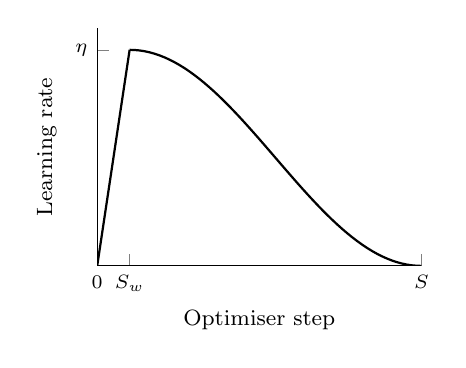
\begin{tikzpicture}
\begin{axis}[width=0.47\linewidth, height=4.6cm, xlabel={Optimiser step}, ylabel={Learning rate},
  label style={font=\footnotesize}, tick label style={font=\scriptsize}, xmin=0, xmax=1, ymin=0, ymax=1.1,
  xtick={0,0.1,1}, xticklabels={$0$,$S_w$,$S$}, ytick={1}, yticklabels={$\eta$}, axis lines*=left]
\addplot[thick, no marks, domain=0:0.1, samples=2] {x/0.1};
\addplot[thick, no marks, domain=0.1:1, samples=60] {0.5*(1+cos(deg(pi*(x-0.1)/0.9)))};
\end{axis}
\end{tikzpicture}\hspace{0.6cm}%
\pendingplot{5.6cm}{loss curves: written from\\results/train\_log.json\\when the training run ends}
\fi
\caption{Left: learning rate, linear warmup over $S_w$ steps to the peak $\eta$, then a half cosine to
zero at the planned last step $S$ (the cosine decay of \citealp{loshchilov2017sgdr}). The planned
schedule runs to step $S=\fyTrainPlannedSteps{}$; the run stopped early at step \fyTrainSteps{}, so the
rest was never used. Recomputed from the run's settings in
\texttt{results/train\_log.json} once it exists (schematic until then). Right: training loss per logged
step and held-out loss per evaluation, from the same log.}
\label{fig:train}
\end{figure}

\subsection{fy-m1 versus the base model}
Table~\ref{tab:results} compares the two models on the test set and the regression checks.

\begin{table}[t]
\centering
\small
\begin{tabular}{lrr}
\toprule
Measure & Base & fy-m1 \\
\midrule
Drift to full French/English ($\downarrow$) & \fyDriftBase & \fyDriftFymOne \\
Naturalness, LLM judge, 1--5 ($\uparrow$) & \fyNaturalBase & \fyNaturalFymOne \\
Correctness, LLM judge, 1--5 ($\uparrow$) & \fyCorrectBase & \fyCorrectFymOne \\
Held-out chat perplexity ($\downarrow$) & \fyPplBase & \fyPplFymOne \\
Belebele accuracy ($\uparrow$) & \fyBelebeleBase & \fyBelebeleFymOne \\
FLORES+ chrF++ mg$\to$en ($\uparrow$) & \fyChrfMgEnBase & \fyChrfMgEnFymOne \\
FLORES+ chrF++ en$\to$mg ($\uparrow$) & \fyChrfEnMgBase & \fyChrfEnMgFymOne \\
\bottomrule
\end{tabular}
\caption{Base model versus fy-m1 on \fyEvalPrompts{} prompts (\texttt{results/eval/scores.json}; judge
rows from \texttt{results/eval/judge.json}). Belebele and FLORES+ are regression checks: they should not
fall much.}
\label{tab:results}
\end{table}

\subsection{Release gates}
\paragraph{Leak gate} (\path{results/eval/scores.json}, \path{results/eval/leak_review.json}).
\fyLeakFymOne{} of fy-m1 answers had a shared 8-word run; there were \fyLeakMatches{} distinct matched
runs, of which \fyLeakGeneric{} were judged generic phrases and \fyLeakRejected{} were rejected.

\paragraph{Identity check} (\path{results/eval/identity_check.json}). fy-m1 passed
\fyIdentityPassed{} of \fyIdentityN{} replies (\fyIdentityPassRate{}; threshold \fyIdentityThreshold{});
hard fails: \fyIdentityForeign{}; gate \fyIdentityGate{}.

\subsection{Blind human comparison (early votes)}
From \path{results/eval/arena.json}: \fyArenaVotes{} votes from \fyArenaRaters{} raters; fy-m1 win rate
\fyArenaWinRate{} (95\% Wilson interval \fyArenaCiLow{}--\fyArenaCiHigh{}; \citealp{wilson1927}).
With so few raters this is a first signal, not a result.

\subsection{Vocabulary trimming}
The public keep set alone is measured (\path{results/shrink/trim_cost.json}): it shrinks the vocabulary
from \fyCostVocabBefore{} to \fyCostVocabAfter{} tokens, and every held-out line decodes back unchanged.
The cost is slightly longer token sequences: tokens per word go from \fyCostTpwChatsBefore{} to
\fyCostTpwChatsAfter{} on the anonymised chats and from \fyCostTpwPromptsBefore{} to
\fyCostTpwPromptsAfter{} on the test prompts. The trimmed model itself (\path{results/shrink.json}): gates
\fyTrimGates{}; vocabulary \fyVocabBefore{} $\to$ \fyVocabAfter{} tokens; parameters \fyParamsBefore{}
$\to$ \fyParamsAfter{}; download \fyGgufBefore{} $\to$ \fyGgufAfter{}; speed on the demo CPU
\fyTpsBefore{} $\to$ \fyTpsAfter{} tokens/s.

\section{Limitations}
\label{sec:limitations}
\begin{itemize}
  \item \textbf{One family.} The real chats come from one family. The style reflects their everyday
        speech, not every region or dialect.
  \item \textbf{Mostly synthetic, from the base model itself.} There are \fySynthGateKept{} synthetic
        chats against \fyGateKept{} real ones, and the generator is the base model. Training a model on
        its own outputs can narrow what it says \citep{shumailov2024collapse}; the few-shot real examples
        carry the new style, but the synthetic chats also carry the base model's habits and mistakes. The
        sample gate checks privacy and form, not quality, and is not a native speaker.
  \item \textbf{Over-masking.} The strict gate replaces rare words and texting spellings with fake names,
        which makes the real chats a little less natural.
  \item \textbf{Automatic evidence first.} The human comparison has only early votes from
        \fyArenaRaters{} raters. Until the full panel is in, the main evidence is automatic.
  \item \textbf{The judge.} An LLM judge may not understand Malagasy slang well; its scores can be wrong
        in either direction, and I have not measured its agreement with native speakers. The judge is a
        closed model, so the judge scores cannot be reproduced exactly with open tools.
  \item \textbf{The drift metric is lenient.} English that contains a Malagasy name or a quoted Malagasy
        word can pass as Malagasy, so the drift rate can be a little low.
  \item \textbf{Small, single-run comparisons.} The greeting gate uses \fyGreetAnswers{} answers per model,
        the base-model comparison is partial (Gemma~4's translation and speed are pending), and training is
        one run with one seed and untuned settings. No difference here comes with a significance test
        except the arena's interval.
  \item \textbf{Word rules for identity.} The identity gate matches word patterns; a false claim in an
        unusual phrasing can pass it.
  \item \textbf{A chat model, not a source of facts.} The model can be slow on a free CPU, get facts
        wrong, and invent things.
\end{itemize}

\section{Ethics}
\label{sec:ethics}
\paragraph{Consent and privacy.} Everyone in the chats agreed to the use of their messages. The pipeline is
built so that no person reads the cleaned text, including me, and so that any doubt drops data instead of
keeping it (Section~\ref{sec:data}). Neither the cleaned chats nor the raw answers are released in v0.1.
Before release, the leak gate checks that the model does not repeat training text, and the public
snapshot of the repository is checked automatically for names and copied chat text. The anonymisation
is not perfect (Section~\ref{sec:data} lists its known gaps); the gates reduce the risk but do not
remove it.

\paragraph{Use of closed models.} No closed-API model output is in the training data. The LLM judge
(disclosed in Section~\ref{sec:metrics}) only scores answers to public prompts and never sees private
text; its outputs are not training data.

\paragraph{Safety.} The model was trained with a small set of polite refusals and gets a basic identity and
safety check before release, but it is not a safety-tested product. A model that chats casually in a
low-resource language is also harder for outside moderators to check, which is one more reason the
model card states its limits plainly.

\section{Future work}
\label{sec:future}
For v0.2:
\begin{itemize}
  \item The full panel's blind human comparison, with confidence intervals, and the judge's agreement
        with it.
  \item Each model's answer to each test prompt.
  \item The layer-pruning experiment.
  \item Longer training, more than one seed, and more everyday data.
  \item A second run (r2) on a new data mix that stops the role-play: synthetic chats cut before any reply
        that plays a person, identity chats repeated, real pairs kept only when the reply answers, and
        human-written Malagasy prompt and answer pairs from the Aya Dataset \citep{singh2024aya}, capped at
        20\% of the mix.
\end{itemize}
After that, two larger steps, in this order:
\begin{enumerate}
  \item \textbf{A bigger curated corpus of everyday Malagasy text.} The main limit of fy-m1 is data: the
        real chats come from one family and most of the volume is synthetic. I plan to build a larger,
        curated and consented collection of everyday Malagasy writing, cleaned with the same strict
        privacy gates.
  \item \textbf{A Malagasy speech model.} Much everyday Malagasy is spoken, not typed. With a stronger
        text model in place, I plan to work on a model that understands and speaks everyday Malagasy.
\end{enumerate}

\section*{Acknowledgements}
\label{sec:ack}
I thank everyone in the chats for agreeing to let me use their messages.

\paragraph{Licence.} fy-m1's weights are released under CC-BY-4.0, the base model's licence
(\fyBaseLicense{}), with attribution to \citet{afriqueqwen}. The code is Apache-2.0. Gemma~3 was used only
as a measured baseline; none of its outputs are in the training data. The formal chats are built from
Malagasy Wikipedia text, which is CC-BY-SA 4.0. I credit it here. The weights stay CC-BY-4.0. Anyone who
reuses Malagasy Wikipedia text must follow its ShareAlike terms.

\paragraph{Base model.} AfriqueQwen3.5-9B-50Langs-Instruct-v1 by McGill-NLP \citep{afriqueqwen},
CC-BY-4.0. Gemma~4 12B \citep{gemma4} (Apache-2.0) and Gemma~3 12B \citep{gemma3} (Gemma Terms of Use)
were comparison rows only.

\paragraph{Data.} Data cleaning uses \texttt{wordfreq} by Robyn Speer \citep{wordfreq} (word data
CC-BY-SA 4.0; derived word lists keep that licence and attribution), word case counts from Malagasy
Wikipedia \citep{wikipedia-dump} (CC-BY-SA 4.0), HPLT 2.0 cleaned Malagasy web text \citep{hplt2}
(CC0-1.0 on its dataset card; I keep only a word list, never the text), and the INSEE first-name file
\citep{insee-prenoms} (Licence Ouverte / Etalab 2.0). The formal slice uses Malagasy Wikipedia.
The r2 mix uses the original (human-written) Malagasy annotations of the Aya Dataset \citep{singh2024aya}
(Apache-2.0). Evaluation uses Belebele \citep{bandarkar-etal-2024-belebele} and FLORES+ \citep{floresplus}, both
CC-BY-SA 4.0 on their dataset cards.

\paragraph{Tools.} Language ID uses GlotLID \citep{kargaran-etal-2023-glotlid}, under the licence terms on
its model card. Training uses Unsloth \citep{unsloth} and Hugging Face Transformers, both Apache-2.0; the
demo runs on llama.cpp (MIT). GPUs: free T4s from Kaggle and Google Colab, and a paid Colab Pro A100.

\bibliographystyle{plainnat}
\bibliography{refs}

\end{document}
